\clearpage
\begin{explanationbox}

	\textbf{\textcolor{CExplanation}{一句话直觉}}

	对数回答的是“把底数乘方多少次，才得到真数”？图像的上升或下降由底数决定；函数值正负还要看真数位于$1$的哪一边。

	\medskip
	

\textbf{\textcolor{CExplanation}{为什么会想到对数函数？}}
\begin{center}\begin{tikzpicture}[font=\small,>=stealth,line join=round]
\draw[gray!40,rounded corners=3pt] (0,0) rectangle (14.2,9.1);\node at (7.1,8.5) {方法一：2的一次方是2，反过来问得到对数};
\begin{scope}[shift={(2.6,3.1)},x=.94cm,y=.94cm]\draw[->,gray] (-1.5,0)--(4.4,0) node[right]{$x$};\draw[->,gray] (0,-1.5)--(0,4.4) node[above]{$y$};\draw[gray,dashed] (-1.3,-1.3)--(4,4);\draw[blue!75!black,thick,domain=.42:4.1,samples=160] plot(\x,{ln(\x)/ln(2)});\draw[violet,thick,dashed,domain=-1.3:2.04,samples=160] plot(\x,{pow(2,\x)});\fill[violet] (1,2) circle(2pt);\fill[blue!75!black] (2,1) circle(2pt);\draw[gray,densely dotted] (1,2)--(2,1);\node[below right=4pt] at (3.2,3.2){$y=x$};\end{scope}\node[anchor=west,text width=5cm,align=left] at (8.5,4.5) {紫虚线：$y=2^x$\\[8pt]蓝实线：$y=\log_2x$\\[8pt]$(1,2)\leftrightarrow(2,1)$\\[8pt]横、纵坐标交换\\[8pt]一般：$(u,v)\leftrightarrow(v,u)$};
\node[text width=12.6cm,align=center] at (7.1,.65) {两轴单位相同；(1,2)与(2,1)交换坐标。几个数字帮助发现规律，不能代替一般证明。};
\end{tikzpicture}\end{center}



学过$2^3=8$后，如果反过来问“$2$要乘方多少次才得到$8$”，答案是$3$，写作$\log_2 8=3$。
对数不是突然出现的新运算，而是\textbf{把指数的结果和次数倒过来求}：
\[
  a^y=x\quad\Longleftrightarrow\quad y=\log_a x
  \qquad(a>0,\ a\ne1,\ x>0).
\]
比如$2^{-1}=\tfrac12$，所以$\log_2\tfrac12=-1$；这说明\textbf{对数的真数一定大于$0$，函数值却可以为负数}。

\medskip

\end{explanationbox}
\clearpage
\begin{explanationbox}
\textbf{\textcolor{CExplanation}{核心拆解}}
\begin{center}\begin{tikzpicture}[font=\small,>=stealth,line join=round]
\draw[gray!40,rounded corners=3pt] (0,0) rectangle (14.2,8.3);\node at (7.1,7.700000000000001) {从指数反求次数：真数只能为正，次数却没有正负限制};
\begin{scope}[shift={(1.6660377358490566,4.1269230769230765)},x=1.1320754716981132cm,y=0.7076923076923076cm]\draw[->,gray] (-0.5,0)--(4.8,0) node[right]{$x$};\draw[->,gray] (0,-3.5)--(0,3) node[above]{$y$};\draw[blue!75!black,thick,solid,domain=0.125:4.2,samples=180] plot(\x,{ln(\x)/ln(2)});\fill[orange!85!black] (0.25,-2) circle(2.2pt);\fill[orange!85!black] (1,0) circle(2.2pt);\fill[orange!85!black] (4,2) circle(2.2pt);\draw[gray,dashed] (.05,-2)--(4.3,-2);\draw[gray,dashed] (.05,2)--(4.3,2);\draw[gray!35,densely dotted] (1,0)--(1,-3.5);\node[below=3pt] at (1,-3.5){$1$};\draw[gray!35,densely dotted] (4,0)--(4,-3.5);\node[below=3pt] at (4,-3.5){$4$};\end{scope}\node[anchor=west,align=left,text width=5.0cm] at (8.4,4.0) {$x=2^y$总大于0\\[8pt]$y=-2\Rightarrow x=\frac14$\\[8pt]$y=0\Rightarrow x=1$\\[8pt]$y=2\Rightarrow x=4$\\[8pt]任意实数$y$都有正数$x$\\[8pt]定义域$(0,+\infty)$，值域$\mathbb R$};
\node[text width=12.6cm,align=center] at (7.1,.65) {水平线y=c与曲线的交点横坐标为2的c次方，总能找到且总为正数。};
\end{tikzpicture}\end{center}


	\begin{description}[style=nextline, leftmargin=2.8em, labelsep=0.5em, itemsep=0.45em]
		\item[\textbf{要点一（定义域限制）：}] 自变量$x$必须大于$0$，所以图像只出现在$y$轴右侧。
		\item[\textbf{要点二（单调性条件）：}] 底数$a>1$时递增，$0<a<1$时递减，是比较大小的基础。
		\item[\textbf{要点三（符号法则）：}] 当$x>1$或$0<x<1$时，结合底数可得$y$的正负。
	\end{description}

	\medskip
	
\end{explanationbox}
\clearpage
\begin{explanationbox}
\textbf{\textcolor{CExplanation}{用五个数字看懂“增、减、过定点”：}}
\begin{center}\begin{tikzpicture}[font=\small,>=stealth,line join=round]
\draw[gray!40,rounded corners=3pt] (0,0) rectangle (14.2,8.8);\node at (7.1,8.200000000000001) {把数表放到曲线上：相同五个真数，输出顺序相反};
\node at (3.1500000000000004,7.3) {$y=\log_2x$};\begin{scope}[shift={(1.092,4.65)},x=0.9800000000000001cm,y=0.6346153846153846cm]\draw[->,gray] (-0.4,0)--(4.6,0) node[right]{$x$};\draw[->,gray] (0,-2.6)--(0,2.6) node[above]{$y$};\draw[blue!75!black,thick,solid,domain=0.2:4.2,samples=180] plot(\x,{ln(\x)/ln(2)});\fill[orange!85!black] (0.25,-2.0) circle(2pt);\fill[orange!85!black] (0.5,-1.0) circle(2pt);\fill[orange!85!black] (1,0.0) circle(2pt);\fill[orange!85!black] (2,1.0) circle(2pt);\fill[orange!85!black] (4,2.0) circle(2pt);\draw[gray!35,densely dotted] (1,0)--(1,-2.6);\node[below=3pt] at (1,-2.6){$1$};\draw[gray!35,densely dotted] (2,0)--(2,-2.6);\node[below=3pt] at (2,-2.6){$2$};\draw[gray!35,densely dotted] (4,0)--(4,-2.6);\node[below=3pt] at (4,-2.6){$4$};\end{scope}\node[align=center,text width=5.8cm] at (3.1500000000000004,1.7) {五点的高度为\\$-2,-1,0,1,2$};\node at (9.95,7.3) {$y=\log_{1/2}x$};\begin{scope}[shift={(7.892,4.65)},x=0.9800000000000001cm,y=0.6346153846153846cm]\draw[->,gray] (-0.4,0)--(4.6,0) node[right]{$x$};\draw[->,gray] (0,-2.6)--(0,2.6) node[above]{$y$};\draw[orange!85!black,thick,dashed,domain=0.2:4.2,samples=180] plot(\x,{ln(\x)/ln(0.5)});\fill[orange!85!black] (0.25,2.0) circle(2pt);\fill[orange!85!black] (0.5,1.0) circle(2pt);\fill[orange!85!black] (1,-0.0) circle(2pt);\fill[orange!85!black] (2,-1.0) circle(2pt);\fill[orange!85!black] (4,-2.0) circle(2pt);\draw[gray!35,densely dotted] (1,0)--(1,-2.6);\node[below=3pt] at (1,-2.6){$1$};\draw[gray!35,densely dotted] (2,0)--(2,-2.6);\node[below=3pt] at (2,-2.6){$2$};\draw[gray!35,densely dotted] (4,0)--(4,-2.6);\node[below=3pt] at (4,-2.6){$4$};\end{scope}\node[align=center,text width=5.8cm] at (9.95,1.7) {相同真数，五点高度为\\$2,1,0,-1,-2$};
\node[text width=12.6cm,align=center] at (7.1,.65) {两图同尺度；五个真数依次为1/4、1/2、1、2、4，具体点只能帮助发现规律。};
\end{tikzpicture}\end{center}


\[
\begin{array}{c|ccccc}
  x & \tfrac14 & \tfrac12 & 1 & 2 & 4\\ \hline
  \log_2 x & -2 & -1 & 0 & 1 & 2\\
  \log_{1/2}x & 2 & 1 & 0 & -1 & -2
\end{array}
\]
从左往右，真数从$\tfrac14$变到$4$；底数为$2$时，需要的指数从$-2$增到$2$；底数为$\tfrac12$时，指数却从$2$减到$-2$。这就解释了两种底数下图像方向相反。\textbf{不论底数是哪一种，$a^0=1$，所以$\log_a1=0$，都经过$(1,0)$。}

\medskip

\end{explanationbox}
\clearpage
\begin{explanationbox}
\textbf{\textcolor{CExplanation}{为什么真数必须大于$0$，函数值却能取一切实数？}}
\begin{center}\begin{tikzpicture}[font=\small,>=stealth,line join=round]
\draw[gray!40,rounded corners=3pt] (0,0) rectangle (14.2,8.3);\node at (7.1,7.700000000000001) {从指数反求次数：真数只能为正，次数却没有正负限制};
\begin{scope}[shift={(1.6660377358490566,4.1269230769230765)},x=1.1320754716981132cm,y=0.7076923076923076cm]\draw[->,gray] (-0.5,0)--(4.8,0) node[right]{$x$};\draw[->,gray] (0,-3.5)--(0,3) node[above]{$y$};\draw[blue!75!black,thick,solid,domain=0.125:4.2,samples=180] plot(\x,{ln(\x)/ln(2)});\fill[orange!85!black] (0.25,-2) circle(2.2pt);\fill[orange!85!black] (1,0) circle(2.2pt);\fill[orange!85!black] (4,2) circle(2.2pt);\draw[gray,dashed] (.05,-2)--(4.3,-2);\draw[gray,dashed] (.05,2)--(4.3,2);\draw[gray!35,densely dotted] (1,0)--(1,-3.5);\node[below=3pt] at (1,-3.5){$1$};\draw[gray!35,densely dotted] (4,0)--(4,-3.5);\node[below=3pt] at (4,-3.5){$4$};\end{scope}\node[anchor=west,align=left,text width=5.0cm] at (8.4,4.0) {$x=2^y$总大于0\\[8pt]$y=-2\Rightarrow x=\frac14$\\[8pt]$y=0\Rightarrow x=1$\\[8pt]$y=2\Rightarrow x=4$\\[8pt]任意实数$y$都有正数$x$\\[8pt]定义域$(0,+\infty)$，值域$\mathbb R$};
\node[text width=12.6cm,align=center] at (7.1,.65) {水平线y=c与曲线的交点横坐标为2的c次方，总能找到且总为正数。};
\end{tikzpicture}\end{center}



把$y=\log_a x$改写为$x=a^y$。底数合规时，不论$y$是正、负还是$0$，$a^y$总大于$0$；因此$x$只能是正数。反过来，任意实数$y$都能算出一个$x=a^y>0$，所以对数的函数值可以取任意实数。

\medskip

\end{explanationbox}
\clearpage
\begin{explanationbox}
\textbf{\textcolor{CExplanation}{两种“对称”不能混为一谈：}}
\begin{center}\begin{tikzpicture}[font=\small,>=stealth,line join=round]
\draw[gray!40,rounded corners=3pt] (0,0) rectangle (14.2,8.3);\node at (7.1,7.700000000000001) {方法三的第一种对称：同一真数，函数值取相反数};
\begin{scope}[shift={(1.589795918367347,3.9499999999999997)},x=1.2244897959183672cm,y=0.7666666666666666cm]\draw[->,gray] (-0.4,0)--(4.5,0) node[right]{$x$};\draw[->,gray] (0,-3)--(0,3) node[above]{$y$};\draw[blue!75!black,thick,solid,domain=0.18:4,samples=180] plot(\x,{ln(\x)/ln(2)});\draw[orange!85!black,thick,dashed,domain=0.18:4,samples=180] plot(\x,{ln(\x)/ln(0.5)});\fill[orange!85!black] (2,1) circle(2.2pt);\fill[orange!85!black] (2,-1) circle(2.2pt);\fill[orange!85!black] (1,0) circle(2.2pt);\draw[gray,dashed] (2,-1)--(2,1);\draw[gray!35,densely dotted] (1,0)--(1,-3);\node[below=3pt] at (1,-3){$1$};\draw[gray!35,densely dotted] (2,0)--(2,-3);\node[below=3pt] at (2,-3){$2$};\draw[gray!35,densely dotted] (4,0)--(4,-3);\node[below=3pt] at (4,-3){$4$};\end{scope}\node[anchor=west,align=left,text width=5.0cm] at (8.4,4.0) {$\log_{1/a}x=-\log_ax$\\[10pt]$(2,1)\leftrightarrow(2,-1)$\\[10pt]横坐标相同\\[10pt]纵坐标互为相反数\\[10pt]对称轴为$x$轴};
\node[text width=12.6cm,align=center] at (7.1,.65) {对称时改变的是纵坐标；一般点(x,t)对应(x,-t)，x仍然大于0。};
\end{tikzpicture}\end{center}



当底数由$2$换成$\tfrac12$，同一个真数$x=2$对应$1$和$-1$，所以两条对数曲线\textbf{关于$x$轴对称}。
但$y=2^x$与$y=\log_2 x$是把“指数”和“结果”倒过来写，例如前者的$(1,2)$对应后者的$(2,1)$，因此\textbf{关于$y=x$对称}。

\begin{center}
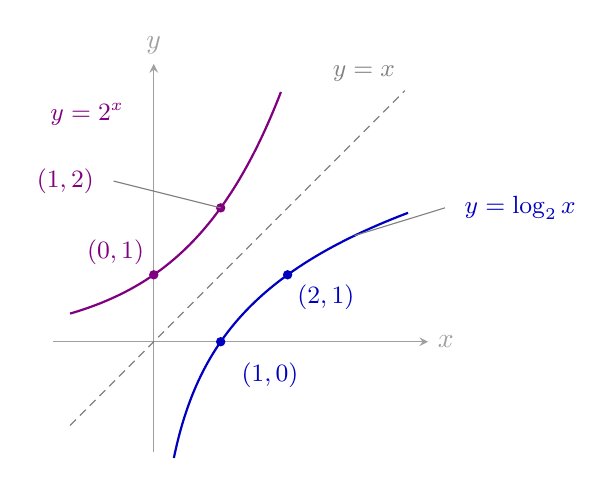
\begin{tikzpicture}[x=0.85cm,y=0.85cm,>=stealth]
  \draw[->,gray!75] (-1.5,0)--(4.1,0) node[right] {$x$};
  \draw[->,gray!75] (0,-1.65)--(0,4.15) node[above] {$y$};
  \draw[densely dashed,gray] (-1.25,-1.25)--(3.75,3.75) node[above left] {\small $y=x$};
  \draw[violet,thick,domain=-1.25:1.9,samples=80,smooth] plot (\x,{exp(ln(2)*\x)});
  \draw[blue!75!black,thick,domain=0.3:3.8,samples=80,smooth] plot (\x,{ln(\x)/ln(2)});
  \fill[violet] (0,1) circle (1.7pt) node[above left] {\small $(0,1)$};
  \fill[blue!75!black] (1,0) circle (1.7pt) node[below right=4pt] {\small $(1,0)$};
  \fill[violet] (1,2) circle (1.7pt);\draw[gray] (1,2)--(-.6,2.4);\node[violet,anchor=east] at (-.75,2.4) {\small $(1,2)$};
  \fill[blue!75!black] (2,1) circle (1.7pt) node[below right] {\small $(2,1)$};
  \node[violet,anchor=east] at (-.3,3.4) {\small $y=2^x$};
  \draw[gray] (3,1.58496)--(4.35,2);\node[blue!75!black,anchor=west] at (4.5,2) {\small $y=\log_2 x$};
\end{tikzpicture}
\par\small 指数与对数把同一对数的顺序交换，例如$(1,2)\leftrightarrow(2,1)$。
\end{center}

\medskip

\end{explanationbox}
\clearpage
\begin{explanationbox}
\textbf{\textcolor{CExplanation}{几何本质（图像接近$y$轴但不碰到）}}
\begin{center}\begin{tikzpicture}[font=\small,>=stealth,line join=round]
\draw[gray!40,rounded corners=3pt] (0,0) rectangle (14.2,8.3);\node at (7.1,7.700000000000001) {曲线可以靠近y轴，却没有x=0这个点};
\begin{scope}[shift={(1.6454545454545455,4.897058823529411)},x=2.1818181818181817cm,y=0.9019607843137255cm]\draw[->,gray] (-0.25,0)--(2.5,0) node[right]{$x$};\draw[->,gray] (0,-3.6)--(0,1.5) node[above]{$y$};\draw[blue!75!black,thick,solid,domain=0.125:2.2,samples=180] plot(\x,{ln(\x)/ln(2)});\fill[orange!85!black] (0.5,-1) circle(2.2pt);\fill[orange!85!black] (0.25,-2) circle(2.2pt);\fill[orange!85!black] (0.125,-3) circle(2.2pt);\draw[gray,dashed] (.125,-3)--(.125,0);\draw[gray!35,densely dotted] (1,0)--(1,-3.6);\node[below=3pt] at (1,-3.6){$1$};\draw[gray!35,densely dotted] (2,0)--(2,-3.6);\node[below=3pt] at (2,-3.6){$2$};\end{scope}\node[anchor=west,align=left,text width=5.0cm] at (8.4,4.0) {$x=\frac12:\ y=-1$\\[9pt]$x=\frac14:\ y=-2$\\[9pt]$x=\frac18:\ y=-3$\\[9pt]每个横坐标都大于0\\[9pt]永远不能令$x=0$};
\node[text width=12.6cm,align=center] at (7.1,.65) {靠近的是x=0这条竖直线，并非经过y轴上的某个点；定义域没有0。};
\end{tikzpicture}\end{center}



	当$x$趋近于$0^+$时，$y$趋近于$-\infty$（$a>1$）或$+\infty$（$0<a<1$），即图像无限接近$y$轴但不相交，$y$轴是垂直渐近线。

	\medskip
	
\end{explanationbox}
\clearpage
\begin{explanationbox}
\textbf{\textcolor{CExplanation}{代数意义（符号映射）}}
\begin{center}\begin{tikzpicture}[font=\small,>=stealth,line join=round]
\draw[gray!40,rounded corners=3pt] (0,0) rectangle (14.2,8.8);\node at (7.1,8.200000000000001) {以(1,0)为分界记符号：大底升，小底降};
\node at (3.1500000000000004,7.3) {$a>1$（图取2）};\begin{scope}[shift={(1.1454545454545455,4.65)},x=1.1136363636363635cm,y=0.5892857142857143cm]\draw[->,gray] (-0.4,0)--(4,0) node[right]{$x$};\draw[->,gray] (0,-2.8)--(0,2.8) node[above]{$y$};\draw[blue!75!black,thick,solid,domain=0.22:3.7,samples=180] plot(\x,{ln(\x)/ln(2)});\fill[orange!85!black] (1,0) circle(2pt);\node at (.5,-1.8){$-$};\node at (3,1){$+$};\draw[gray!35,densely dotted] (1,0)--(1,-2.8);\node[below=3pt] at (1,-2.8){$1$};\end{scope}\node[align=center,text width=5.8cm] at (3.1500000000000004,1.7) {$0<x<1$：负\\$x>1$：正};\node at (9.95,7.3) {$0<a<1$（图取1/2）};\begin{scope}[shift={(7.945454545454545,4.65)},x=1.1136363636363635cm,y=0.5892857142857143cm]\draw[->,gray] (-0.4,0)--(4,0) node[right]{$x$};\draw[->,gray] (0,-2.8)--(0,2.8) node[above]{$y$};\draw[orange!85!black,thick,dashed,domain=0.22:3.7,samples=180] plot(\x,{ln(\x)/ln(0.5)});\fill[orange!85!black] (1,0) circle(2pt);\node at (.5,1.8){$+$};\node at (3,-1){$-$};\draw[gray!35,densely dotted] (1,0)--(1,-2.8);\node[below=3pt] at (1,-2.8){$1$};\end{scope}\node[align=center,text width=5.8cm] at (9.95,1.7) {$0<x<1$：正\\$x>1$：负};
\node[text width=12.6cm,align=center] at (7.1,.65) {两图同尺度；把函数值与0比较，等于把真数与1比较，再按底数决定方向。};
\end{tikzpicture}\end{center}



	从$y=\log_a x$看：$a>1$时，真数在$1$右边，函数值为正；在$1$左边，函数值为负。$0<a<1$时恰好相反。记住$(1,0)$这条分界线，不必死记四个符号。

	\medskip
	
\end{explanationbox}
\clearpage
\begin{explanationbox}
\textbf{\textcolor{CExplanation}{沿水平线识别底数（补充图解）}}
\begin{center}\begin{tikzpicture}[font=\small,>=stealth,line join=round]
\draw[gray!40,rounded corners=3pt] (0,0) rectangle (14.2,8.3);\node at (7.1,7.700000000000001) {沿水平线看底数：上方交点右移、下方交点也右移};
\begin{scope}[shift={(1.475,3.9499999999999997)},x=0.9375cm,y=0.9199999999999999cm]\draw[->,gray] (-0.4,0)--(6,0) node[right]{$x$};\draw[->,gray] (0,-2.5)--(0,2.5) node[above]{$y$};\draw[blue!75!black,thick,solid,domain=0.24:5.5,samples=180] plot(\x,{ln(\x)/ln(2)});\draw[violet,thick,dashed,domain=0.24:5.5,samples=180] plot(\x,{ln(\x)/ln(3)});\draw[orange!85!black,thick,densely dotted,domain=0.24:5.5,samples=180] plot(\x,{ln(\x)/ln(0.5)});\draw[teal,thick,dashdotted,domain=0.24:5.5,samples=180] plot(\x,{ln(\x)/ln(0.3333333333333333)});\fill[orange!85!black] (2,1) circle(2.2pt);\fill[orange!85!black] (3,1) circle(2.2pt);\fill[orange!85!black] (2,-1) circle(2.2pt);\fill[orange!85!black] (3,-1) circle(2.2pt);\fill[orange!85!black] (1,0) circle(2.2pt);\draw[gray,dashed] (.2,1)--(5.6,1);\draw[gray,dashed] (.2,-1)--(5.6,-1);\draw[->,black,thick] (2.15,1)--(2.85,1);\draw[->,black,thick] (2.15,-1)--(2.85,-1);\draw[gray!35,densely dotted] (1,0)--(1,-2.5);\node[below=3pt] at (1,-2.5){$1$};\draw[gray!35,densely dotted] (2,0)--(2,-2.5);\node[below=3pt] at (2,-2.5){$2$};\draw[gray!35,densely dotted] (3,0)--(3,-2.5);\node[below=3pt] at (3,-2.5){$3$};\draw[gray!35,densely dotted] (5,0)--(5,-2.5);\node[below=3pt] at (5,-2.5){$5$};\end{scope}\node[anchor=west,align=left,text width=5.0cm] at (8.4,4.0) {蓝$\log_2x$，紫$\log_3x$\\[8pt]橙$\log_{1/2}x$，青$\log_{1/3}x$\\[8pt]在$y=1$上：$x=a$\\[5pt]向右：底数$2\to3$增大\\[8pt]在$y=-1$上：$x=1/a$\\[5pt]向右：底数$\frac12\to\frac13$减小};
\node[text width=12.6cm,align=center] at (7.1,.65) {先确认选的是y=1还是y=-1；同样向右移动，对应底数的变化方向恰好相反。};
\end{tikzpicture}\end{center}

\textbf{读图与使用：}$y=1$时$x=a$；$y=-1$时$x=1/a$。上方交点右移表示底数增大；下方右移表示底数减小。

\textbf{\textcolor{CExplanation}{考点价值（高频考点）}}
	\begin{itemize}[leftmargin=*, itemsep=0.5em, topsep=0.4em]
		\item \textbf{考法一（比较大小）：} 利用单调性比较同底对数式，或借助中间量$0$、$1$比较不同底对数。
		\item \textbf{考法二（定义域求解）：} 求对数型函数的定义域，必须保证真数大于$0$。
	\end{itemize}

	\medskip
	\textbf{\textcolor{CExplanation}{顿悟点}}

\textbf{真数的正负限制来自指数恒为正；上升还是下降来自底数；函数值的正负来自底数与真数相对$1$的位置。}所以做题先查真数是否为正，再看底数，最后比较大小。

	\medskip
	\textbf{\textcolor{CExplanation}{使用场景}}
	\begin{itemize}[leftmargin=*, itemsep=0.5em, topsep=0.4em]
		\item \textbf{场景一（比较大小）：} 同底时直接比较真数；不同底时化为同底或使用中间值。
		\item \textbf{场景二（解对数不等式）：} 利用单调性转化为真数的不等式，同时注意定义域。
\end{itemize}

\medskip
\textbf{\textcolor{CExplanation}{什么时候最快？}}

题目出现“两个同底对数比大小”“含参数底数的不等式”“函数图像经过哪一点”“图像关于哪条直线对称”时，不要先计算小数；用真数范围、底数分类、$(1,0)$和坐标交换，往往一步就能判断。
\end{explanationbox}
